\documentclass[author-year, 12pt,review]{components/elsarticle} %review=doublespace preprint=single 5p=2 column
%%% Begin My package additions %%%%%%%%%%%%%%%%%%%
\usepackage[hyphens]{url}
\usepackage{lineno} % add 
  \linenumbers % turns line numbering on 
\bibliographystyle{elsarticle-harv}
\biboptions{sort&compress} % For natbib
\usepackage{graphicx}
\usepackage{booktabs} % book-quality tables
%% Redefines the elsarticle footer
\makeatletter
\def\ps@pprintTitle{%
 \let\@oddhead\@empty
 \let\@evenhead\@empty
 \def\@oddfoot{\it \hfill\today}%
 \let\@evenfoot\@oddfoot}
\makeatother

% A modified page layout
\textwidth 6.75in
\oddsidemargin -0.15in
\evensidemargin -0.15in
\textheight 9in
\topmargin -0.5in
%%%%%%%%%%%%%%%% end my additions to header

\usepackage[T1]{fontenc}
\usepackage{lmodern}
\usepackage{amssymb,amsmath}
\usepackage{ifxetex,ifluatex}
\usepackage{fixltx2e} % provides \textsubscript
% use upquote if available, for straight quotes in verbatim environments
\IfFileExists{upquote.sty}{\usepackage{upquote}}{}
\ifnum 0\ifxetex 1\fi\ifluatex 1\fi=0 % if pdftex
  \usepackage[utf8]{inputenc}
\else % if luatex or xelatex
  \usepackage{fontspec}
  \ifxetex
    \usepackage{xltxtra,xunicode}
  \fi
  \defaultfontfeatures{Mapping=tex-text,Scale=MatchLowercase}
  \newcommand{\euro}{€}
\fi
% use microtype if available
\IfFileExists{microtype.sty}{\usepackage{microtype}}{}
\usepackage{graphicx}
% We will generate all images so they have a width \maxwidth. This means
% that they will get their normal width if they fit onto the page, but
% are scaled down if they would overflow the margins.
\makeatletter
\def\maxwidth{\ifdim\Gin@nat@width>\linewidth\linewidth
\else\Gin@nat@width\fi}
\makeatother
\let\Oldincludegraphics\includegraphics
\renewcommand{\includegraphics}[1]{\Oldincludegraphics[width=\maxwidth]{#1}}
\ifxetex
  \usepackage[setpagesize=false, % page size defined by xetex
              unicode=false, % unicode breaks when used with xetex
              xetex]{hyperref}
\else
  \usepackage[unicode=true]{hyperref}
\fi
\hypersetup{breaklinks=true,
            bookmarks=true,
            pdfauthor={},
            pdftitle={Do we need detailed demographic data to forecast plant population responses to climate change?},
            colorlinks=true,
            urlcolor=blue,
            linkcolor=magenta,
            pdfborder={0 0 0}}
\urlstyle{same}  % don't use monospace font for urls
\setlength{\parindent}{0pt}
\setlength{\parskip}{6pt plus 2pt minus 1pt}
\setlength{\emergencystretch}{3em}  % prevent overfull lines
\setcounter{secnumdepth}{0}
% Pandoc toggle for numbering sections (defaults to be off)
\setcounter{secnumdepth}{0}
% Pandoc header



\begin{document}
\begin{frontmatter}

  \title{Do we need detailed demographic data to forecast plant population
responses to climate change?}
    \author[usu]{Andrew T. Tredennick\corref{c1}}
   \ead{atredenn(at)gmail.com} 
   \cortext[c1]{Corresponding author}
    \author[usu]{Peter B. Adler}
  
  
      \address[usu]{Department of Wildland Resources and the Ecology Center, Utah State
University, Logan, UT 84322, USA}    
  
  \begin{abstract}
  Forecasts of populations under future climate change are constrained by
  the spatial and temporal scales at which we can gather data. For plants,
  ecologists often require individual level data to build population
  models; data that is difficult and expensive to collect at spatial
  scales greater than one square meter. Models built using such data are
  difficult to scale-up to spatial scales relevant to land management
  decisions and policy intervention. A possible route forward are
  density-structured models based on coarse-scale census data, which are
  much easier to collect over large spatial extents. However, to use
  coarse-scale data in a climate change context requires the assumption
  that the climate signals in population dynamics identified using
  individual-level data can also be identified when individual-level data
  are averaged over. Here we use a longterm dataset to model population
  dynamics using individual-level and plot-level data.
  \end{abstract}
   \begin{keyword} ecological forecasts \sep population models \sep integral projection model \sep climate change \sep grassland \sep \end{keyword}
 \end{frontmatter}


\section{Introduction}\label{introduction}

Population models are important tools for predicting the impacts of
environmental change on species. But reconciling the scales at which
population models are parameterized and the scales at which
environmental changes play out remains a challenge (Freckleton et al.
2011, Queenborough et al. 2011). The major hurdle is that most
population models, at least for plant species, are built using data from
small, localized plots because parameterizing traditional population
models requires tracking the fates of individuals. These models are
difficult to scale up from the micro to meso-scales because the fitted
parameters do not fully represent the spatial variation present scales
beyond that at which the data are collected (Sæther et al. (2007)).
Thus, our ability to use population models to predict the consequences
of climate change is limited.

Recently, Freckleton et al. (2011), building on work by Hastings and
NAME, have proposed density-structured population models that focus on
the transition of populations among discrete states, rather than the
traditional approach of modeling the transitions of individuals. Such an
approach could be extremely valuable because the data needed to
parameterize density-structured population models is much easier, and
less costly, to collect (Queenborough et al. year). For example, using a
density-structured approach, one could build a population model using a
time series of annual plot-based censuses of species percent cover.
However, a major assumption of the density-structured approach is that
the aggregate dynamics of the population observed at coarse spatial
resolution faithfully represent, and correspond to, the fates of
individual plants. In other words, using a density-structured approach
requires a leap of faith that important covariates (e.g., climate
variables) at the level of the individual are captured adequately at the
population level. If we seek to forecast the impacts of climate change
on plant populations, then clearly this assumption requires testing.

\section{Materials and Methods}\label{materials-and-methods}

\subsubsection{Study site and data}\label{study-site-and-data}

Our demographic data comes from the Fort Keogh Livestock and Range
Research Laboratory in eastern Montana's northern mixed prairie near
Miles City, Montana, USA (46 deg. 19' N, 105 deg 48' W). The dataset is
freely available on Ecological Archives (CITE), and interested readers
should refer to the metadata therin for a complete description. The site
is about 800 m above sea level and mean annual precipitation (1878-2009)
is 334 mm, with most annual precipitaion falling from April through
September (76). The site is grass dominated and, for the purposes of our
study, we focus on the four most abundant graminoid species:
\emph{Bouteloua gracilis}, \emph{Hesperostipa comata},
\emph{Pascopyrum smithii}, and \emph{Poa secunda}.

From 1932 to 1945 individual plants were identified and mapped annualy
in 44 1-m2 quadrats using a pantograph. The quadrats were distributed in
six pastures, each assigned a grazing treatment of light (1.24 ha/animal
unit month), moderate (0.92 ha/aum), and heavy (0.76 ha/aum) stocking
rates (two pastures per treatment). In this analysis we account for
potential differences among the grazing treatments, but do not focus on
grazing$\times$climate interactions. The annual maps of the quadrats
were digitized and the fates of individual plants tracked and extracted
using a computer program. Daily climate data, which we aggregated into
climate variables of interest, are available for the duration of the
data collection period (1932 - 1945) from the Miles City airport, Wiley
Field, 9 km from the study site.

\subsubsection{Stastical models of vital
rates}\label{stastical-models-of-vital-rates}

The first step in building our single-species population models was to
fit statistical models of vital rates at both levels of inference:
individual-level and quadrat-level. Here we describe the general
statistical approach at the individual-level, but the same approach
applies at the quadrat-level. We modeled survival and growth as
functions of genet size (quadrat cover in the quadrat-level models) and
climate covariates (described in more detail below). We maintained a
consistent random effects structure for both models that included three
terms: (1) a random year effect on the intercept, (2) a random year
effect on the coefficient for plant cover (either individual or quadrat
level), and (3) a random effect of group (see Data set description) on
the intercept. Vital rates for each species are modeled separately.

We used logistic regression to model survival probability:

\begin{equation}
logit(s) = \beta_{0,t} + \beta_{s,t}x + \beta_{Q} + \beta_{c,1}\theta_{1,t}\\
+ \cdots +  \beta_{c,i}\theta_{i,t} + \varepsilon_{t}
\end{equation}

where $x$ is the log of genet size (quadrat areal cover), $\beta_{0,t}$
is a year-specific intercept, $\beta_{s,t}$ is the year-specific slope
parameter for size, $\beta_{Q}$ is the random effect of quadrat group
location, $\theta$ is a matrix of $i$ climate effects over $t$ years,
$\beta_{c,i}$ is the fixed parameter for the effect of the $i$th climate
covariate, and $\varepsilon_{t}$ is the error term. At the quadrat level
we did not fit random year effects for survival because those parameters
did not reach convergence (see ``Computing'').

We modeled growth as gaussian process describing genet size (or quadrat
cover) at time $t+1$ as a function of size at $t$ and climate
covariates:

\begin{equation}
x_{t+1} = \beta_{0,t} + \beta_{s,t}x_{t} + \beta_{Q} + \beta_{c,1}\theta_{1,t}\\
+ \cdots +  \beta_{c,i}\theta_{i,t} + \varepsilon_{t}
\end{equation}

where $x$ is genet size and all other paramters are as described for the
survival regression. For the quadrat-level approach we modeled growth as
a process describing proportional cover within a quadrat at time $t+1$
as a function of proportional cover at time $t$ and climate covariates.
Thus, instead of a gaussian process, with a normal likelihood, we
modeled growth at the quadrat level as above but with a beta likelihood
and a logit link to the linear predictors.

While our approach for modeling survival and growth is similar at the
individual and quadrat levels, the addition of new genets at the
inidividual level or occupied sites at the quadrat level requires two
separate approaches.

\subsubsection{Including climate covariates (and avoiding model
selection)}\label{including-climate-covariates-and-avoiding-model-selection}

For both the individual-level IPM (IPM) and the quadrat-based IBM (QBM)
we included four climate covariates in each vital rate regression: fall
through spring precipitation at \emph{t}-1 and \emph{t}-2 (ppt1 and
ppt2, respectively) and mean spring temperature at \emph{t}-1 and
\emph{t}-2 (TmeanSpr1 and TmeanSpr2, respectively), where \emph{t} is
the observation year. We included climate covariates as additive
effects. We did not consider interactions among climate covariates or
among climate covariates and plant size or proportional cover. Climate
effects ($\beta_{c}$s) were modeled hierarchically in each vital rate
regression so that each species specific climate effect is drawn from an
interspecific climate effect distribution. This was necessary to achieve
convergence at the quadrat level and we used the same approach at the
individual level for uniformity.

\subsubsection{Model fitting}\label{model-fitting}

All of our analyses (model fitting and simulating) were conducted in
Program R. We used the MCMC sampler in JAGS to estimate the posterior
distributions of model parameters. We obtained posterior distributions
for all model parameters from three parallel MCMC chains run for 50,000
iterations, after a 50,000 iteration burn in. We assessed convergence
visually and using the Gelman diagnostic in the R package `coda.' Scale
reduction factors for all parameters were less than 1.02, indicating
convergence. For the purposes of introducing stochasticity in our
population models, we saved the final 1,000 iterations from each chain
for all parameters to be used as randomly drawn values during population
simulation.

\subsubsection{Population models}\label{population-models}

With the posterior distribution of the vital rate statistical models in
hand, it is straightforward to simulate the population models.

\section{Results}\label{results}

We assessed the statistical importance of the climate covariates
included the final vital rate regressions by comparing the residual
deviance of models with climate covariates and temporal random effects,
climate covariates only, and temporal random effects only. When a model
includes climate covariates, this comparison shows the relative
contribution of the climate covariates in explaining the total
interannual variability (Adler et al. (2012)).

\begin{figure}[htbp]
\centering
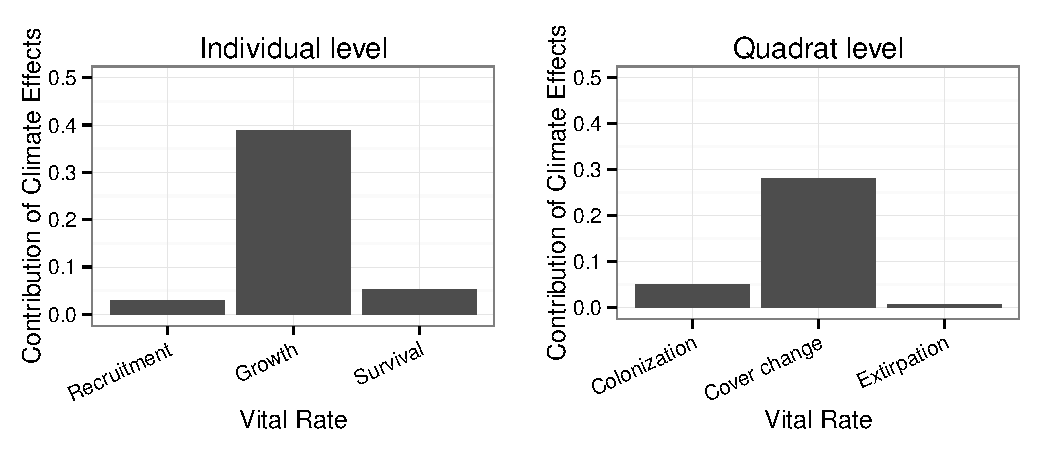
\includegraphics{components/figure/manuscript-figure_1.pdf}
\caption{The proportion of interannual variability in vital rates
explained by the climate covariates. The contribution for growth is
defined as: (Climate model - Constant Model)/(Full model - Constant
model). The contribution for survival and colonization, where we could
not estimate a full model with year random effects at the quadrat level,
is defined as: (Constant Model - Climate Model)/Constant Model.}
\end{figure}

\begin{figure}[htbp]
\centering
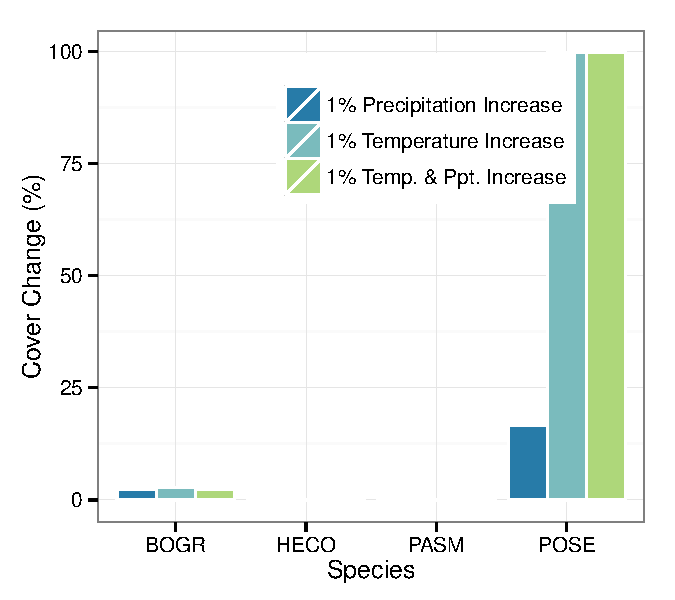
\includegraphics{components/figure/manuscript-figure_2.pdf}
\caption{Posterior means (vertical ticks), 75\% credible intervals
(heavy lines), and 95\% credible intervals (light lines) of climate
effects on growth at both levels of inferences. The dashed vertical line
is at 0, indicating no effect. Horizontal line at 0 indicates perfect
agreement between mean observed cover in that year and the model
predictions.}
\end{figure}

\begin{figure}[htbp]
\centering
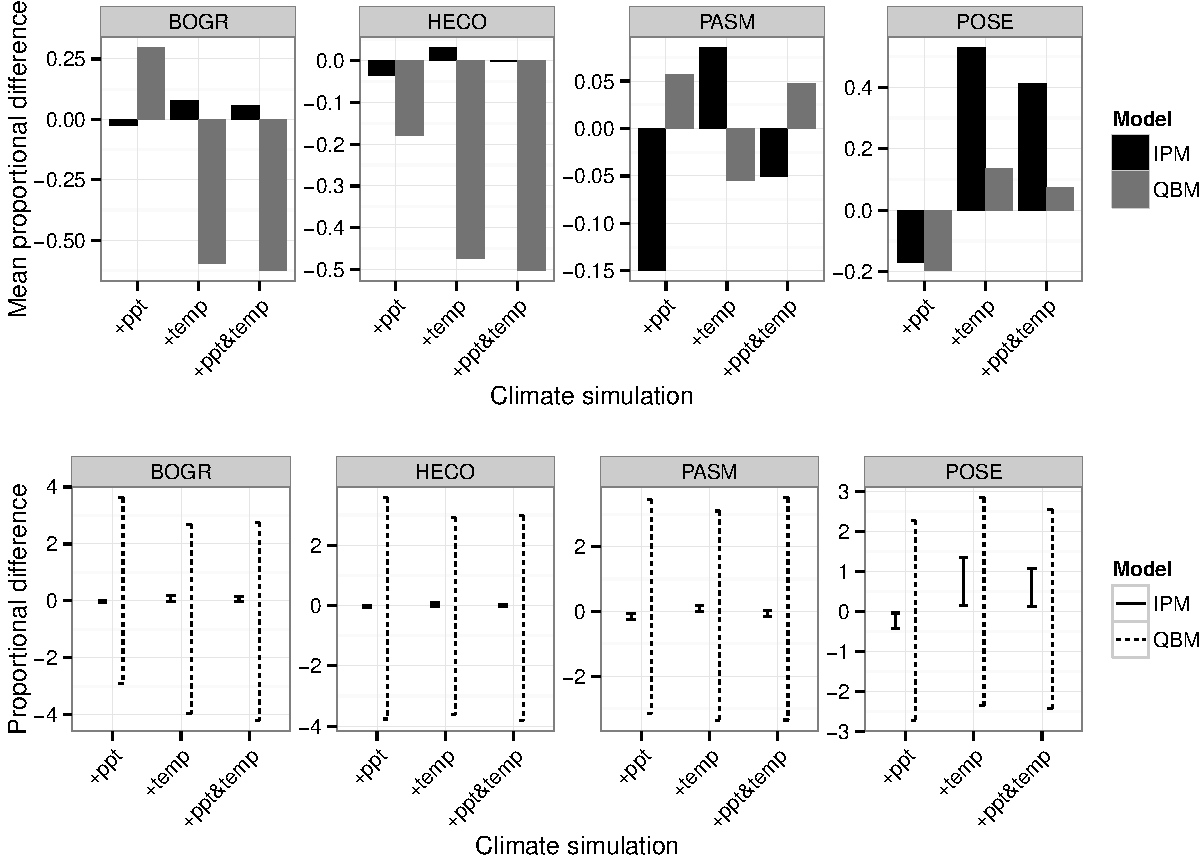
\includegraphics{components/figure/manuscript-figure_3.pdf}
\caption{Boxplots of model residuals for one-step-ahead forecasts at
each observation year. Each one-step forecast was simulated
\texttt{r nSims} times. Note that the y-axes vary across panels. The
light blue line shows the difference between the observed-year percent
cover and the average cover observed across all years. The models tend
to underpredict and perform poorly when observed cover in a given year
is a large deviant from the mean.}
\end{figure}

\begin{center}\rule{3in}{0.4pt}\end{center}

\section{References}\label{references}

Adler, P. B., H. J. Dalgleish, and S. P. Ellner. 2012. Forecasting plant
community impacts of climate variability and change: when do competitive
interactions matter? Journal of Ecology 100:478--487.

Freckleton, R. P., W. J. Sutherland, A. R. Watkinson, and S. A.
Queenborough. 2011. Density-structured models for plant population
dynamics. American Naturalist 177:1--17.

Queenborough, S. A., K. M. Burnet, W. J. Sutherland, A. R. Watkinson,
and R. P. Freckleton. 2011. From meso- to macroscale population
dynamics: A new density-structured approach. Methods in Ecology and
Evolution 2:289--302.

Sæther, B. E., S. Engen, V. Grøtan, W. Fiedler, E. Matthysen, M. E.
Visser, J. Wright, A. P. Møller, F. Adriaensen, H. {Van Balen}, D.
Balmer, M. C. Mainwaring, R. H. McCleery, M. Pampus, and W. Winkel.
2007. The extended Moran effect and large-scale synchronous fluctuations
in the size of great tit and blue tit populations. Journal of Animal
Ecology 76:315--325.

\end{document}


